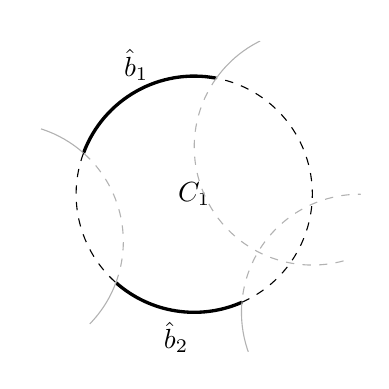
\begin{tikzpicture}[
    scale=1.5,
    >=stealth,
    point/.style = {draw, circle,  fill = black, inner sep = 1pt},
    dot/.style   = {draw, circle,  fill = black, inner sep = .2pt},
  ]
  	
	\coordinate (R1) at (3.2,4); % Mittelpunkt des ersten Kreises
	\coordinate (R2) at (1.6,3.6); % Mittelpunkt des zweiten Kreises
	\coordinate (R3) at (4.2,4.4); % Mittelpunkt des dritten Kreises
	\coordinate (R4) at (4.6,3); % Mittelpunkt des vierten Kreises
	
	\clip(R1)circle[x radius=1.41, y radius=1.41];
	% Kreismittelpunkte
	\node (M1) at (R1) [label = {center:$C_1$}]{};
	
	% Bögen
	% C1
	\draw[very thick] (R1) ++(79.22:1) arc (79.22:159.59:1) node[midway, above]{$\hat{b}_1$};
	\draw[very thick] (R1) ++(228.49:1) arc (228.49:293.81:1) node[midway, below]{$\hat{b}_2$};
	\draw[dashed] (R1) ++(159.59:1) arc (159.59:228.49:1);
	\draw[dashed] (R1) ++(293.81:1) arc (293.81:439.22:1);
	
	% C2
	\draw[gray!60] (R2) ++(48.49:1) arc (48.49:339.59:1) node[midway, left]{$C_2$};
	\draw[dashed,gray!60] (R2) ++(339.59:1) arc (339.59:408.49:1);
	
	% C3
	\draw[gray!60] (R3) ++(329.23:1) arc (329.23:504.38:1) node[midway, above right]{$C_3$};
	\draw[dashed,gray!60] (R3) ++(144.38:1) arc (144.38:329.23:1);
	
	% C4
	\draw[gray!60] (R4) ++(175.12:1) arc (175.12:422.67:1) node[midway, below right]{$C_5$};
	\draw[dashed,gray!60] (R4) ++(62.67:1) arc (62.67:175.12:1);
	
\end{tikzpicture}